% ----- formatovani dokumentu -----------------------------------------------
\documentclass[12pt,a4paper,titlepage,final]{report}
\usepackage[utf8]{inputenc}
\usepackage[T1, IL2]{fontenc}
\usepackage{graphicx}
\usepackage{epstopdf}
\usepackage[margin=2cm]{caption}
\usepackage[top=3cm, left=2cm, right=2cm, text={17cm, 24cm}, ignorefoot]{geometry}
\usepackage{color}
\usepackage{url}
\usepackage{setspace}
\singlespacing
\usepackage[square, numbers]{natbib}
\pagestyle{plain}
\pagenumbering{arabic}
\setcounter{page}{1}
\setcounter{secnumdepth}{-1}
\setlength{\parindent}{1cm}
\usepackage{natbib}


% ----- vyberte jazyk -------------------------------------------------------
\usepackage[english,czech]{babel}
%\usepackage[english]{babel}

% ----- dopiste titulky -----------------------------------------------------
\newcommand\Course{Počítačová grafika}
\newcommand\WorkTitle{Realistické generování oblohy}
\newcommand\AuthorA{Miloslav Číž}
\newcommand\AuthorAEmail{xcizmi00@stud.fit.vutbr.cz}
\newcommand\AuthorB{Aleš Dujíček}
\newcommand\AuthorBEmail{xdujic01@stud.fit.vutbr.cz}
\newcommand\Faculty{Fakulta Informačních Technologií}
\newcommand\School{Vysoké Učení Technické v Brně}

\usepackage[
pdftitle={\WorkTitle},
pdfauthor={\AuthorA, \AuthorB},
bookmarks=true,
colorlinks=true,
breaklinks=true,
urlcolor=blue,
citecolor=blue,
linkcolor=blue,
unicode=true,
]
{hyperref}


% ----- titulni strana ------------------------------------------------------

\begin{document}
    \begin{titlepage}
    \begin{center}
        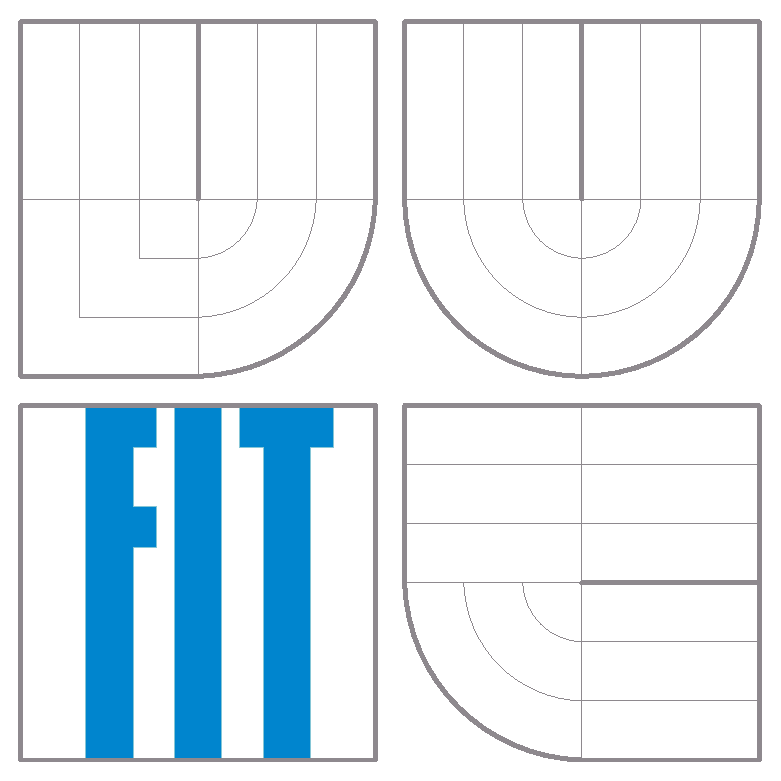
\includegraphics[height=5cm]{images/logo.eps}
    \end{center}
    \vfill
    \begin{center}
        \begin{Large}
            \Course\\
        \end{Large}
        \bigskip
        \begin{Huge}
            \WorkTitle\\
        \end{Huge}
    \end{center}
    \vfill
    \begin{center}
        \begin{large}
            \today
        \end{large}
    \end{center}
    \vfill
    \begin{flushleft}
        \begin{large}
            \begin{tabular}{lll}
                Autoři: & \AuthorA, & \url{\AuthorAEmail} \\
                        & \AuthorB, & \url{\AuthorBEmail} \\
                & & \\
                & \Faculty \\
                & \School \\
            \end{tabular}
        \end{large}
    \end{flushleft}
\end{titlepage}

% ----- obsah --------------------------------------------------------------

\tableofcontents

% ----- zadani -------------------------------------------------------------
\newpage
\chapter{Zadání}

Zadáním bylo vytvořit program pro vhodně parametrizovatelné generování realistických obrázků oblohy za použití vhodné metody (založené např. na sledování paprsku). Měli jsme se zaměřit na vizuální kvalitu oblohy, krajinu stačilo vykreslit pouze velmi zjednodušeně. Zadání jsme upřesnili následujícím způsobem:

\begin{itemize}
    \item generování obrázků oblohy podobných fotografii
    \item metoda: sledování paprsku v kombinaci s 2D vykreslováním
        \item procedurální generování textury mraků
        \item možnost generovat sekvenci obrázků jako animaci (volitelně navazující)
\end{itemize}

%---------------------------------------------------------------------------
\chapter{Nejdůležitější dosažené výsledky}

Popište 3 věci, které jsou na vašem projektu nejlepší. Nejlépe ukažte a
komentujte obrázky, v nejhorším případě vypište textově.

\section{První věc}

Lorem ipsum dolor sit amet, consectetur adipiscing elit. In non condimentum augue, quis accumsan tellus. Sed sagittis mauris tortor, a varius ipsum feugiat sed. Morbi dapibus neque purus, id condimentum sem tincidunt quis. Sed lacinia a justo in rutrum. Nam a enim id urna cursus consectetur non a mi. Fusce vitae augue urna. Nunc nec malesuada enim, vitae blandit leo. Vestibulum et orci nibh. Phasellus in nisi rutrum, mattis metus vehicula, tempus neque.

\begin{itemize}
    \item Položka 1
    \begin{itemize}
        \item Podpoložka 1.1
        \item Podpoložka 1.2
        \item $\ldots$
    \end{itemize}
    \item Položka 2
    \item $\ldots$
\end{itemize}

\begin{center}
    \captionsetup{type=figure}
        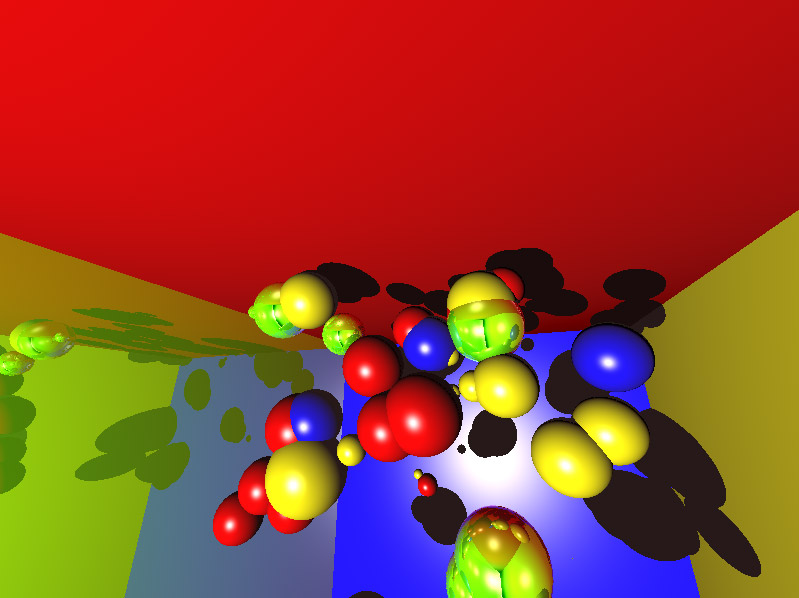
\includegraphics[width=10cm]{images/sample.jpg}
    \captionof{figure}{Popisek vzorového obrázek}
\end{center}

\section{Druhá věc}

Etiam a laoreet dolor, vel blandit ipsum. Pellentesque habitant morbi tristique senectus et netus et malesuada fames ac turpis egestas. Nam aliquet ipsum eget semper pretium. Maecenas mauris tortor, pretium sit amet convallis et, iaculis vel tortor. Donec ultrices magna et commodo tempus. Etiam sagittis lectus vitae lectus ultricies tincidunt. Nam aliquam non magna eget pellentesque.

\begin{table}[h!]
    \begin{center}
    \begin{tabular}{ | p{3.5cm} | p{3.5cm} | p{3.5cm} | p{3.5cm} |}
    \hline
    Sloupec A & Sloupec B & Sloupec C & Sloupec D
    \\ \hline

    A1 & B1 & C1 & D1
    \\ \hline

    A2 & B2 & C2 & D2
    \\ \hline

    \end{tabular}
    \end{center}
    \caption{Vzorová tabulka}
\end{table}

\section{Třetí věc}

Vestibulum ac tellus et massa facilisis tristique in in ante. In elementum luctus ante, id cursus nulla. Quisque sit amet dolor dui. Suspendisse bibendum auctor augue, a posuere enim dictum non. Nunc iaculis libero eget interdum egestas. Suspendisse pretium cursus massa vel fringilla.



%---------------------------------------------------------------------------
\chapter{Zvláštní použité znalosti}

Uveďte informace, které byly potřeba nad rámec výuky probírané na FIT.
Vysvětlete je pomocí obrázků, schémat, vzorců apod.

\paragraph{Rozsah:} podle potřeby a vlastního uvážení


%---------------------------------------------------------------------------
\chapter{Práce na projektu}

\begin{itemize}
\item \textbf{\AuthorA}: implementace sledování paprsku, vykreslení pozadí a krajiny
\item \textbf{\AuthorB}: implementace Perlinova šumu
\end{itemize}

%---------------------------------------------------------------------------
\section{Co bylo nejpracnější}

Popište, co vám při řešení nejvíce komplikovalo život, s čím jste se museli
potýkat, co zabralo čas.

\paragraph{Rozsah:} 5-10 řádků

\begin{itemize}
\item \textbf{\AuthorA}: Prácné bylo todle a tamto.
\item \textbf{\AuthorB}: Pracné bylo vyvážit poměr kafe, mléka a cukru.
\end{itemize}


%---------------------------------------------------------------------------
\section{Zkušenosti získané řešením projektu}

Popište, co jste se řešením projektu naučili. Zahrňte dovednosti obecně
programátorské, věci z oblasti počítačové grafiky, ale i spolupráci v týmu,
hospodaření s časem, atd.

\paragraph{Rozsah:} formulujte stručně, uchopte cca 3-5 věcí

%---------------------------------------------------------------------------
\chapter{Autoevaluace}

Ohodnoťte vaše řešení v jednotlivých kategoriích (0 – nic neuděláno,
zoufalství, 100\% – dokonalost sama). Projekt, který ve finále obdrží plný
počet bodů, může mít složky hodnocené i hodně nízko. Uvedení hodnot blízkých
100\% ve všech nebo mnoha kategoriích může ukazovat na nepochopení problematiky nebo na snahu kamuflovat slabé stránky projektu. Bodově hodnocena bude i
schopnost vnímat silné a slabé stránky svého řešení.

\paragraph{Technický návrh (50\%):} (analýza, dekompozice problému, volba
vhodných prostředků, $\ldots$)
Stručně (1-2 řádky) komentujte hodnocení.

\paragraph{Programování (50\%):} (kvalita a čitelnost kódu, spolehlivost běhu,
obecnost řešení, znovupoužitelnost, $\ldots$)
Stručně (1-2 řádky) komentujte hodnocení.

\paragraph{Vzhled vytvořeného řešení (50\%):} (uvěřitelnost zobrazení,
estetická kvalita, vhled GUI, $\ldots$)
Stručně (1-2 řádky) komentujte hodnocení.

\paragraph{Využití zdrojů (50\%):} (využití existujícího kódu a dat, využití
literatury, $\ldots$)
Stručně (1-2 řádky) komentujte hodnocení.

\paragraph{Hospodaření s časem (50\%):} (rovnoměrné dotažení částí projektu,
míra spěchu, chybějící části řešení, $\ldots$)
Stručně (1-2 řádky) komentujte hodnocení.

\paragraph{Spolupráce v týmu (50\%):} (komunikace, dodržování dohod, vzájemné
spolehnutí, rovnoměrnost, $\ldots$)
Stručně (1-2 řádky) komentujte hodnocení.

\paragraph{Celkový dojem (50\%):} (pracnost, získané dovednosti, užitečnost,
volba zadání, cokoliv, $\ldots$)
Stručně (5-10 řádků) komentujte hodnocení.

%---------------------------------------------------------------------------
\chapter{Ovládání vytvořeného programu}

\section{Technologie potřebné pro spuštění programu}
Zde vypište, jaké technologie vaše řešení používá – co potřebuje k běhu, co
jste použili při tvorbě, atd. Text strukturujte, použijte odrážky,
číslování$\ldots$

\paragraph{Rozsah:} odrážky, dle potřeby

\section{Programy a služby použité při tvorbě}
Zde vypište, jaké technologie vaše řešení používá – co potřebuje k běhu, co
jste použili při tvorbě, atd. Text strukturujte, použijte odrážky,
číslování$\ldots$

\paragraph{Rozsah:} odrážky, dle potřeby

\section{Obsluha programu}
Stručně popište, jak se program ovládá (nejlépe odrážky rozdělené do
kategorií). Pokud se ovládání odchyluje od zkratek a způsobů obvykle
používaných v okýnkových nadstavbách operačních systémů, zdůvodněte, proč se
tak děje.

\paragraph{Rozsah:} odrážky nebo jednoduchý popis a odrážky


%---------------------------------------------------------------------------
\chapter{Doporučení pro budoucí zadávání projektů}

Co vám vyhovovalo a co nevyhovovalo na organizaci projektů? Které prvky by měly být zachovány, zesíleny, potlačeny, eliminovány?

%---------------------------------------------------------------------------

\chapter{Různé}

Ještě něco by v dokumentaci mělo být? Napište to sem! Podle potřeby i založte
novou kapitolu.

%---------------------------------------------------------------------------

\bibliographystyle{plain}

\nocite{cite1}
\nocite{cite2}
\nocite{cite3}

\bibliography{reference}
\addcontentsline{toc}{chapter}{Literatura}

\end{document}

